\documentclass[12pt,letterpaper, onecolumn]{exam}
\usepackage{amsmath}
\usepackage{amssymb}
\usepackage[lmargin=71pt, tmargin=1.2in]{geometry}
\usepackage{graphicx}%For centering solution box
\lhead{IND ENG 221\\}
\rhead{Kartikeya Sharma\\}
% \chead{\hline} % Un-comment to draw line below header
\thispagestyle{empty}   %For removing header/footer from page 1

\begin{document}

\begingroup  
    \centering
    \LARGE IND ENG 221\\
    \LARGE HW 1\\[0.5em]
    \large \today\\[0.5em]
    \large Kartikeya Sharma\par
    \large SID: 3037376860\par
\endgroup
\rule{\textwidth}{0.4pt}
\pointsdroppedatright   %Self-explanatory
\printanswers
\renewcommand{\solutiontitle}{\noindent\textbf{Ans:}\enspace}   %Replace "Ans:" with starting keyword in solution box

\begin{questions}

    \question What is the monthly payment for a 5 year car loan of \$ 20,000with 10\% fixed interest rate (monthly compounding)? Assume 5 x 12 = 60 equal monthly payments
    
    \begin{solution}
        The monthly payment for the 5-year car loan can be calculated using the formula:

\[
M = \frac{P \cdot r \cdot (1 + r)^n}{(1 + r)^n - 1}
\]

Where:
- \( P = 20,000 \) (principal loan amount),
- \( r = \frac{10\%}{12} = 0.00833 \) (monthly interest rate),
- \( n = 5 \times 12 = 60 \) (total number of monthly payments).

Substituting the values:

\[
M = \frac{20000 \cdot 0.00833 \cdot (1 + 0.00833)^{60}}{(1 + 0.00833)^{60} - 1}
\]

After calculating:

\[
M \approx 424.94
\]

Thus, the monthly payment is approximately \$424.94.

    \end{solution}

    \newpage
    \question Suppose that the 6-month, 12-month, 18-month, and 24-month zero rates are 5\%, 6\%, 6.5\%, and 7\%, respectively, with semiannual compounding. What is the 2-year par yield? (The par yield for a certain bond maturity is the coupon rate that causes the bond price to equal its par value (= the notional value.). Assume the bond pays coupon semi-annually. (Hull 4.22)

    \begin{solution}
            The 2-year par yield can be calculated using the formula:

\[
\text{Price} = \frac{c}{2} \times \left( \frac{1}{(1 + r_1)^{0.5}} + \frac{1}{(1 + r_2)^{1}} + \frac{1}{(1 + r_3)^{1.5}} + \frac{1}{(1 + r_4)^{2}} \right) + \frac{100}{(1 + r_4)^{2}}
\]

Where:
- \( r_1 = 5\% \) (6-month rate),
- \( r_2 = 6\% \),
- \( r_3 = 6.5\% \),
- \( r_4 = 7\% \) (24-month rate).

Solving for the par yield \( c \), we find:

\[
\text{Par Yield} \approx 6.84\%
\]

    \end{solution}

    \pagebreak %Not necessary
    
    \question Suppose that risk-free zero interest rates with continuous compounding are as above:
    Calculate forward interest rates for the second, third, fourth, and fifth years. (Hull 4.23)
    
    \begin{figure}
        \centering
        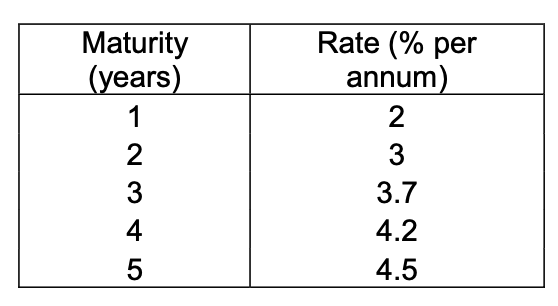
\includegraphics[width=.5\linewidth]{tbl.png}
        \caption{tbl}
        \label{fig:enter-label}
    \end{figure}

    \begin{solution}
            The forward interest rates for the second, third, fourth, and fifth years are calculated as follows:

\[
f_{t, t+1} = \frac{tR_t - (t-1)R_{t-1}}{1}
\]

Where \( R_t \) are the zero rates for time \( t \).

Thus, the forward interest rates are:

\[
\begin{aligned}
f_{1,2} &= 3\% \\
f_{2,3} &= 4.4\% \\
f_{3,4} &= 5.2\% \\
f_{4,5} &= 5.4\%
\end{aligned}
\]

    \end{solution}

    \newpage
    \question The cash prices of 6-month and 1-year Treasury bills are 94.0 and 89.0. A 1.5-year Treasury bond that will pay coupons of \$4 every 6 months currently sells for \$94.84. A 2-year Treasury bond that will pay coupons of \$5 every 6 months currently sells for \$97.12.Calculate the 6-month, 1-year, 1.5-year, and 2-year Treasury zero rates. (Hull 4.29)

    \begin{solution}
            The calculated Treasury zero rates are as follows:

\[
\begin{aligned}
\text{6-month zero rate} &= 12.77\% \\
\text{1-year zero rate} &= 12.36\% \\
\text{1.5-year zero rate} &= 14.19\% \\
\text{2-year zero rate} &= 19.36\%
\end{aligned}
\]

    \end{solution}

\newpage
    \question An interest rate is quoted as 5\% per annum with semiannual compounding. What is the equivalent rate with (a) annual compounding, (b) monthly compounding, and (c) continuous compounding. (Hull 4.34)

    \begin{solution}
     The equivalent interest rates can be calculated by adjusting for the different compounding periods. 
We start with a given rate of 5\% per annum with semiannual compounding.

1. **For annual compounding**, we use the formula:

\[
(1 + \frac{r_{semi}}{2})^2 = (1 + r_{annual})
\]

The equivalent annual rate is:

\[
r_{annual} \approx 5.06\%
\]

2. **For monthly compounding**, we use the formula:

\[
(1 + \frac{r_{semi}}{2})^{2/12} = (1 + \frac{r_{monthly}}{12})
\]

The equivalent monthly compounding rate (annualized) is:

\[
r_{monthly} \approx 4.95\%
\]

3. **For continuous compounding**, we use the formula:

\[
r_{cont} = \ln(1 + \frac{r_{semi}}{2})^2
\]

The equivalent continuous compounding rate is:

\[
r_{cont} \approx 4.94\%
\]
       
    \end{solution}

    
\end{questions}
\end{document}